\chapter{Diagnostics tools, measurements processes \& experimental setup}
This is a "methods" chapter. Its first section presents the available beam diagnostics at the storage ring and describes the experimental measurements of relevant quantities such as beam positions, trajectories and orbits, beam current and lifetime, the tunes and chromaticity and how these are dialed at our will during a study. The last two sections discuss the choice of objective functions to probe the Dynamic Aperture and the appropriate selection of sextupole families as the optimzation knobs.
\section{Diagnostics and measurements at the control room}
\subsection{Beam Position Monitors}
To probe the beam's position along the ring, a diagnostic tool consisting on a set of four pick-up antennas placed within the vaccum chamber are used. These are known as Beam-position-monitors (BPMs), and are sketched in the Figure. The antennas are placed in such a manner so the electron beam deposits mirror charges when passing by then and triggers the antenna a certain voltage signal. The determination of the beam displacements is based on the differential signal induced on the antennas when the beam is not at the geometric center, in which case the induced charges are equal. The signal of the antennas is processed in the so-called "Delta/Sigma" scheme, which gives the horizontal and vertical beam displacements according to the following algebra:
\begin{equation}
    x = K_x \frac{(A+D)-(B+C)}{\Sigma}, \quad y = K_y \frac{(A+B)-(C+D)}{\Sigma},
\end{equation}
where $A,B, C,D$ refers to the intensity of the induced signal over the corresponding antenna, $\Sigma=A+B+C+D$ is the sum signal, proportional to the beam's current, and $K_x$ and $K_y$ are calibration factors, which depend  on the BPM geometry  and distances between the antennas. SIRIUS has 160 BPMs distributed along the storage ring. They allow for the determination of the centroid's positions at a turn-by-turn acquisition rate, which is needed for probing of the betatron motion. The signal can also be processes in other acquisition rates, which renders an averaging of the singal and allows to probe information about the orbit.
\begin{figure}
    \centering
    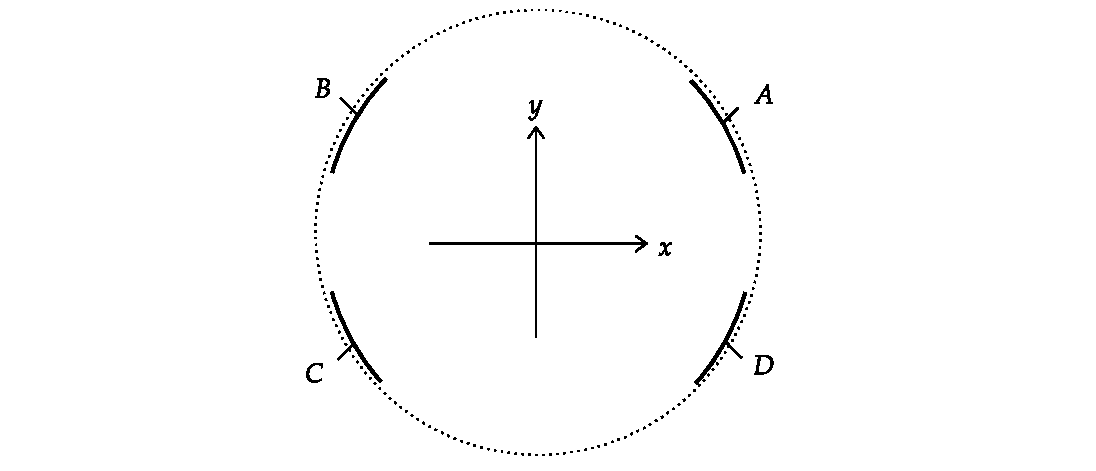
\includegraphics[width=\textwidth]{Images/bpm_scheme.pdf}
    \caption{Schematic representation of BPM button antennas, in solid lines, the vaccum chamber cross-section, in dashed lines, and the transverse positions reference frame.}
    \label{fig:bpms_scheme}
\end{figure}
\subsubsection{Phase-space reconstruction}
Given that BPMs can record TbT motion of the beam's centroid the $x, y$ positions can be readily acquired. The angles, or momenta, can be obtained by the following simple processing. If two consecutive BPMs are located at the ends of a straight section of length $\ell$, where no bending or focusing happens, we can calulate the beam angle as $x^\prime = \frac{\delta x}{\ell}$, where $\Delta x$ refers to the difference of the position readings from the BPMs. On a turn-by-turn basis, the $x,x^\prime$ and $y, y^\prime$ phase-spaces can be reconstructed, as exemplified by Figures below.
\missingfigure{phase space reconstructions}
\subsubsection{Decoherence}
At first sight it might seem the transverse postions are being damped. In fact, the radiative damping time is much bigger then the acquired time scale in the figure, which contains about 300 turns. The radiative damping time for the SIRIUS storage ring is about thousands of turns. This apparent damping a manifestation of the beam's \textit{decoherence}.
Decoherence arises due to the nonlinear tune-shifts and the finite extent of the beam in 6-dimensional phase-space, which implies that there is a spread over transverse amplitudes abd energy deviations. The amplitude-dependent and momentum-dependent tune-shifts render the bunch with a spread in tunes. An initially localized bunch in phase-space quickly filaments and spreads over because of the different frequencies (the tunes). The positions become completely uncorelated and the average of the distribuition, the beam's centroid, goes to zero.
\missingfigure{phase space decoherence}
\subsection{Beam Current and Injection Efficiency}
Direct-Current Current Transformers (DCCTs) enable the measurement of the stored beam current within accelerator rings (booster or storage ring). A DCCT current monitor works by surrounding the the beam of charged particles in the accelerator ring with a magnetic core. The magnetic field induced by the beam current flowing by the core is then measured, allowing for an accurate determination of the current itself.

 Utilizing the current measurement and the beam revolution period in the respective ring, one can assess the stored charge, and calculate the injection efficiency during storage ring injections. By estimating the charge in the booster or transport line just before injection into the storage ring and the storage ring charge immediately after the injection pulse, is possible to deduce the efficiency of the injection process.The efficiency of the injection can also be estimated from the sum-signal of the BPMs, since it is proportional to the stored current.
\todo[inline]{what is the accuracy and prcision of the current measurements with the DCCT? what are its limitations? what about the sum-signal}

\subsection{Tunes measurement \& control}
When turn-by-turn motion is viewed at a fixed longitudinal position $s$, it consits on the sampling of a harmonic motion. Its fundamental frequency is the tune $\nu$. Any observation of Turn-by-turn (TbT) motion can reveal the tunes upon the appropriate singal processing. For instance, the betatron motion can be Fourier-transformed (discrete Fourier transform via fast-fourier transform algorithm), revealing the BPM signal spectrum. Alternatively the time-domain singal can be fitted to a sinusoid, allowing the determination of the tune as the fundamental frequency.

Precise measurement and online monitoring of the tunes in an accelerator ring can be achieved with the aid of a stripline shaker, which constantly drives the beam with an alternating electric field in a narrow of frquencies, leading to sub-nanometer displacements and inducing small-amplitude, noninterfering with operation betatron motion. The same system also reads back the beam response at that same frequency range. The peak of the beam response signal is identified with the betatron tune.
\missingfigure{FFT of betatron motion and shaker spectrum}

As for changing and manipulating the tunes, formula~\eqref{eq:delta_nu} reveals that changes in the quadrupoles strengths, specially at the quadrupoles at large $\beta$-function sections, allow for the control of the tunes.  Since the tune response to quadrupole strength changes is linear, a tune-response matrix can be constructed, i.e. the Jacobian of the tunes with respect to changes in quadrupoles, so that tune changes can be expressed as
\begin{equation}
    \Delta\boldsymbol{\nu} = \vb{J}_{\boldsymbol{\nu}}\Delta \vb{K},
\end{equation}
where $\Delta\boldsymbol{\nu} = \mqty*[\Delta \nu_x & \Delta \nu_y]^\intercal$ is the tune-shifts vector, $\Delta \vb{K}$ is the vector containing the changes in stregths across all the quadrupole families, and the Jacobian or response matrix has entries
\begin{equation}
    (\vb{J}_{\boldsymbol{\nu}})_{ij} = \pdv{\nu_{i}}{K_j} \approx \frac{\Delta \nu_{i}}{\Delta K_j}, \quad i=x, y,\quad j\in\text{quadrupole families}.
\end{equation}
The system can pseudo-inverted, allowing for the determination of quadrupoles changes required for a desired tune change
\begin{equation}
    \Delta \vb{K} = \vb{J}_{\nu}^{+}\Delta \boldsymbol{\nu}
\end{equation}
where $\vb{J}_{\nu}^{+} = (\vb{J}_{\nu}^{\intercal}\vb{J}_{\nu})^{-1}\vb{J}_{\nu}^{\intercal}$ is the Moore-Penrose pseudoinverse.
\todo[inline]{which families are used when changing tunes? add discussion on chaging the optics when changing tunes}
\subsection{Chromaticity measurements \& control}
Chromaticity characterizes the energy-dependent tune-shift. To measure it, we need to calculate the numerical derivative
$$\xi_u = \pdv{\nu_u}{\delta}\approx \frac{\Delta \nu_u}{\delta},$$
that is, measure the tune-shift $\Delta \nu_u$ induced by the energy-shift $\delta$. A direct manner to induce a particular energy-shift is to change the RF cavities frequency (see anexxes for brief overview of longitudinal dynamics and details about momentum compaction). A relation can be established between energy deviations $\delta$ and relative RF frequency changes with the aid of a quantity $\alpha$, known as \textit{momentum compaction factor} \cite{lee_accelerator_2004,sands_physics_1969}:
\begin{equation}
    \delta = -\frac{1}{\alpha}\frac{\Delta f}{f}.
\end{equation}
The momentum compaction factor relates changes in orbit length with energy deviations and is defined by
\begin{equation}
    \alpha = \frac{1}{L}\oint G(s) \eta(s) \dd{s}.
\end{equation}
Therefore, in practice, when measuring chromaticity we are interested in the numerical derivative
\begin{equation}
\xi_u = -\frac{f}{\alpha}\frac{\Delta \nu_u}{\Delta f}
\end{equation}
which is obtained as the first-degree coefficient (properly normalized by $\alpha/f$) of the polynomial fitting of the tune-shift vs. RF frequency curve. A typical tune-shift curve is shown by Fig.
\missingfigure{energy tune shift and chromaticity meas}

As eq.~\eqref{eq:chromaticity} shows, chromaticity depends linearly on the chromatic sextupole families strengths. It can thus be dialed to certain desired values according to the same pseudo-inversion procedure described above for the tunes. We relate the chromaticity changes $\Delta \boldsymbol{\xi}\in\mathbb{R}^2$ to the sextupole families strength changes $\Delta \vb{S}\in\mathbb{R}^{d_s}$ by
\begin{equation}
    \Delta\boldsymbol{\xi} = \vb{J}_{\boldsymbol{\xi}}\Delta \vb{S},
\end{equation}
where $\Delta\boldsymbol{\xi} = \mqty*[\Delta \xi_x & \Delta \xi_y]^\intercal$ and the Jacobian matrix $\vb{J}\in\mathbb{R}^{2 \times d_s}$ has entries
\begin{equation}
    (\vb{J}_{\boldsymbol{\xi}})_{ij} = \pdv{\xi_{i}}{S_j} \approx \frac{\Delta \xi_{i}}{\Delta S_j},\quad i=x, y, \quad j\in\text{sextupole families}.
\end{equation}
$d_s$ refers to cardinality of the set of sextupole families used in the chromaticity change process. In principle, at least two families are required for correcting/tuning chromaticity in the machine: one family for each plane. Since the chromatic sextupole families are the only ones effectively changing chromaticity to leading order, then, at most, $d_s=15$.

If we wish to change chromaticity by a $\Delta\boldsymbol{\xi}$ amount, the jacobian can be pseudo-inverted to calculate the required sextupole strength changes:
\begin{equation}
    \Delta \vb{S} = \vb{J}_{\xi}^{+}\Delta \boldsymbol{\xi}.
\end{equation}

In practice the chromaticity jacobian was never actually measured in the real machine, due to the time-consuming process of varying a single sextupole family, carrying out the chromaticity measurement and repeating the processs for the 15 chromatic families. The "measurement" is instead carried out in the SIRIUS storage ring computer model. The model-calculated jacobian renders a satisfactory correction or tuning of the chromaticity in the actual machine.
\todo[inline]{which families are used for correctiing}
\section{The choice of objective function \& optimzation knobs}

\subsection{The objective function}
\label{subsec:objective_function}
There is no analytical formula relating the storage ring linear or nonlinear optics to the Dynamic Aperture (DA). The optimization procedure must be a heuristic search procedure: changes are performed to the knobs (nonlinear magnets) and the effect on the DA is evaluated. Additionally, one cannot measure the DA in a practical and straightforward measurement procedure sufficiently fast to be run online. Direct measurements of DA can take several iterations of acquiring trajectories of the beam with increasingly higher transverse displacements. The acquisitions are then processed to access the DA. For online optimzation, one must choose a practical, easy-to-measure objective function to act as a probe to the DA: a figure of merit related to the dynamic aperture to represent it and to be used to evaluate the quality of the changes performed during the online tuning process.

In our experiments, we studied using two practical objectives as the probes for DA: the \textbf{injection efficiency} and the \textbf{beam's resilience to dipolar perturbations}. The former is quite self-explanatory: the larger the dynamic aperture, larger the space for the beam to be captured into the storage ring during the injection pulse, and thus the larger the injection efficiency. The latter is related to the DA by the following: the larger the horizontal dipolar kicks the beam can survive, the larger the orbit distortions towards the positive or negative horizontal plane (depending on the kick direction). So the larger the amplitudes the beam explores as it oscillates, probing the DA borders. If the beam survives to large kicks, it means the ring can accomodate larger orbit distortions because of an increased DA.

\missingfigure{ilustrate the injection scheme and the dipole kicks}
% \subsection{Injection scheme for acummulation at SIRIUS storage ring}
% Beam acummulation into the storage ring occurs in the off-axis scheme. The beam is delivered at $x\approx-8~\unit{mm}$, and receives the kick from the nonlinear kicker field. The field profile is nonlinear, with zero field and gradient at the center of the axis, so that it does not disturbs the stored beam.
% In the off-axis scheme, a sufficiently large dynamic aperture is desired to allow the beam to be captured into the storage ring. The predicted efficiency for SIRIUS setup, considering a dynamic aperture reaching $x=-9~\unit{mm}$, was nearly $100\%$. What was observed during 2022 was an injection efficiency of about $88\pm8\%$.

In summary, the dynamic aperture optimization procedure must consist on the exploration of sextupole (knobs) configurations yielding the largest dynamic aperture as accessed by as objective function such as injection efficiency or beam kick-resiliency.

\subsection{The optimization knobs}
\label{subsec:knobs}
The DA is determined by the quality of the beam dynamics in terms of perturbations. Given that a linear optics correction scheme is already in place and regularly implemented in the machine, effectively addressing optics functions and phase advances, the primary factor impacting SIRIUS DA likely stems from nonlinear dynamics and/or remaining uncorrected and previously inaccessible deviations and errors. This may include sextupole field errors or other minor nonlinear multipoles.

If the limitation of the DA is likely associated with nonlinear dynamics, the actuation knobs must unexpectedly be composed of the controllable nonlinear magnets available at the SIRIUS storage ring, namely the sextupoles. However, it is important to note that sextupole strengths cannot be changed arbitrarily. Sextupoles are originally introduced into the lattices as actuators for correcting chromaticity, which refers to the energy-dependent aberrations in the focusing of the beam. Care must be taken when varying the sextupole strengths, as it can alter the chromaticity. A strategy needs to be devised to select the sextupole family in a way that allows for the simultaneous correction of chromaticity and the online tuning of magnet strengths to optimize the DA. In simpler terms, the optimization processes for DA should be conducted while preserving the machine's chromaticity. The natural question that arises is how to implement these isochromatic changes to the sextupoles.

SIRIUS has 21 sextupole families: magnets powered by the same power supply. 6 of them are achromatic sextupoles. They are placed where the the dispersion is zero. The 15 other families are chromatic families. Table~\ref{fams} shows the 21 sextupole families names.
 \begin{table}[htb]
    \caption{SIRIUS sextupole families}
    \centering
    \begin{tabular}{cl}
            \hline
            achromatic & \begin{tabular}[c]{@{}l@{}}SFA0, SDA0, \\ SFB0, SDB0,\\ SDP0, SFP0\end{tabular}                                                                \\ \hline
            chromatic  & \begin{tabular}[c]{@{}l@{}}SDA1, SFA1, \\ SDA2, SFA2, \\ SDA3,\\ SDB1, {SFB1}\\ SDB2, SFB2, \\ SDB3, \\ {SFP1}, SDP1,\\ SDP2, SFP2\\ SDP3\end{tabular} \\ \hline
            \end{tabular}
            \label{fams}
            \end{table}
\todo[inline]{add figure of each family for a superperiod, add the number of magnets for each family}

In principle, thus, the optimization parameter space is 21-dimensional. In reality, as mentioned, we would like to change sextupoles without changing chromaticity. Since we need at least one degree of freedom for correcting chromaticity in the horizontal plane and one degree of freedom for correcting the chromaticity in vertical plane, there are 19 independent knobs available. The dimensionality of the search space can be further reduced by imposing additional constraints to certain families variations.

Throughout the experiments, two strategies were adopted to select the sextupole optimzation knobs. A comapensation scheme and the constrained-families Jacobian null-space knobs.

\subsubsection{Compensation scheme}
\label{subsubsec:compensation}
The idea is the following: out of the 15 chromatic sextupole families, at least two of them are labeled "correction" or "compensation" families and are not freely varied by the optimization routine during the experiment. The other 13 chromatic families can be varied arbitrarily, respecting their linear magnetic (non-saturated) regime. Alongside these 13 chromatic families, the strength of the 6 achromatic sextupole families are also free knobs.  Everytime the routine proposes changes in the free knobs, the chromaticity changes caused by this action are anticipated as follows: the reduced Jacobian, $\tilde{\vb{J}}_\xi$, whose columns contain only those corresponding to the free knobs, is used to calculate the chromaticity change $\Delta \boldsymbol{\xi}=\tilde{\vb{J}}_\xi\Delta\vb{S}_{\text{free}}$ upon the change $\Delta\vb{S}_{\text{free}}$ in the free knobs. Another reduced Jacobian, $\vb{J}_{\xi}^{\prime}$ containig only the columns corresponding to the "correction" or "compensation" families is used to counteract the predicted chromaticity build-up, i.e., to produce sextupole changes $\Delta\vb{S}_{\text{corr.}}$ leading to exactly the oposite chromtaticity change $-\Delta \boldsymbol{\xi}$. The required strength changes in the compensation families is determined by $\Delta \vb{S}_{\text{corr.}} = \vb{J}_{\xi}^{\prime +}(-\Delta \boldsymbol{\xi}$). Applying $\Delta \vb{S} = \Delta \vb{S}_{\text{free.}} + \Delta \vb{S}_{\text{corr.}}$ to the machine leads to sextupole families strength changes keeping the chromaticity unchanged.

In the experiments, the compensation scheme was used as follows. The 6 achromatic families plus the SDA1, SFA1, SDB1, SDP1, SDA3, SDB3 and SDP3 families could be freeely varied. Their strengths were the optimzation knobs. The SDA2, SDB2, SDP2, SFA2, SFB2 and SFP2 were used as the compensation or correction families. They would only be changed so to cancel the chromaticity build-up caused by changing the knobs. The compensation families were chosen on the basis of having range to act on the chromaticity, that is, they were the families with initial strengths far from saturation, with a lot of room to compensate the knobs effects on chromaticity.

\missingfigure{diagram for the compensation scheme}
\subsubsection{Jacobian nullspace-knobs scheme}
\label{subsubsec:nullspace}
Here the idea is to identify the combination of sextupole families living in the nullspace, or kernel, of the chromaticity Jacobian matrix. That is, we are intereseted in the set of vectors $\text{ker}(\vb{J}_\xi)=\text{span}\{\vb{s}_i\in\mathbb{R}^{21}| \vb{J}_{\xi} \vb{s}_i = \vb{0}, i=1,\dots,19 \}$. If we perform changes along such subspace $\Delta \vb{S}\in\text{ker}(\vb{J}_\xi)$ then the resulting changes in chromaticity are null. The resaon why we can anticipate the dimsension of the nullspace is 19 is because it contains the 6 achromatic sextupole families plus 13 degrees of fredom out of the 15 achromatic families, since at least 2 degrees of freedom are needed to act over chromaticity.

A straightforward way to identify the nullspace of the jacobian is to calulate its full singular value decomposition (SVD), which expresses the jacobian as the product
\begin{equation}
    \begin{aligned}
        \vb{J}_\xi &= \vb{U}\boldsymbol{\Sigma}\vb{V}^\intercal\\
                   &= \underbrace{\mqty[\vdots & \vdots \\
                            \vb{u}_1 & \vb{u}_2\\
                            \vdots & \vdots]}_{2\times 2}
                            \underbrace{\mqty[\sigma_1 & 0 & \dots & 0\\
                                             0 & \sigma_2 & \dots & 0 ]}_{2\times21}
                            \underbrace{\mqty[
                                \dots & \vb{v}^\intercal_1 & \dots\\
                                \dots & \vb{v}^\intercal_2 & \dots\\
                                \dots & \vb{v}^\intercal_3 & \dots\\
                                      & \vdots &    \\
                                \dots & \vb{v}^\intercal_{21} & \dots\\                              ]}_{21\times21}.
    \end{aligned}
\end{equation}
Note that the singular-values matrix has only two non-vaninshing singular values $\sigma_1$ and $\sigma_2$. In the sum-over-modes form of SVD, we have
\begin{equation}
    \vb{J}_\xi = \sum_{i=0}^{21}\sigma_i\vb{u}_i\vb{v}_{i}^{\intercal} = \sigma_1 \vb{u}_1\vb{v}_{1}^\intercal + \sigma_2 \vb{u}_2\vb{v}_{2}^\intercal
\end{equation}
in which it is clear that we have only two independent modes or degrees of freedom for changing chromaticity, corresponding to the horizontal and vertical degrees of freedom.

Given the interpretation that the column vectors of the $\vb{U}$ matrix, the so-called right-singular vectors, span the Jacobian row-space, the chromaticity space, and that the row vectors of the $\vb{V}^\intercal$ matrix, the left-singular vectors, span the Jacobian column-space, the sextupole families space, then we can esily identify the vectors living in the nullspace of the Jacobian. They must be the ones associated with the vaninshing singular values: $\text{ker}(\vb{J}_\xi) = \text{span}\{\vb{v}_i|i=3,\dots,21\}$, since changes performed along these directions result in no contribution to the chromaticity.

The discussion above considers no constraints imposed to the sextupole families. In practice, we have also tested imposing additional constraints on the families stretngths variations to further reduce the dimensionality of the search space. For instance, in one of the experiments the following constraints were imposed:
\begin{itemize}
    \item Families SFP1 and SFB1 were kept constant, i.e., were not allowewd to change. They operate close to their saturation, nonlinear regime, and one cannot trust they would be able to provide reproducible magnetic field changes. Deciding not using them already reduces from 21 possible families to 19.
    \item The pair of families SDB1 \& SDP1, SDB2 \& SDP2, SFB2 \& SFP2, SDB3 \& SDP3 were constrained to change by the same amount, starting from their respective initial strengths. This reduces from 19 to 15 degrees of freedom.
\end{itemize}
These 15 families consist on the 6 achromatic families, the 4 pairs of constrained families and 5 other non-constrained families SDA1, SFA1, SDA2 , SFA2, and SDA3. The Jacobian is recalulated and calculating its nullspace reveals the 7-dimensional space spanned by the linear combination of sextupole strengths that when varied will not change chromaticity. We shall refer to such constraint configuration as Constraints Scheme I, to distinguish it from Constraints Scheme II, which consists on
\begin{itemize}
    \item Families SFP1 and SFB1 were kept constant, by the same reason as in the previous scheme.
    \item No pair-wise constraints were imposed to the sextupole families. So, in priciple, there were 19 possible degrees of freedom: 21 minus the two families not used.
\end{itemize}
Calulating the Jacobian nullspace revealed the 17 chromaticity-preserving free knobs.
% \subsection{Characterization of Sextupole Magnets Configurations}
% Once a configuration of sextupoles (position in parameter space) is found, the nonlinear optics it provides the machine needs to be characterized. The characterizations consisted on evaluatig/measuring the followint figures of merit and desired features
% \begin{itemize}
%     \item Injection efficiency in nominal off-axis conditions : this is the most desired characteristic. The sextupoles are to be optimized so the DA and the off-axis injection efficiency increase.
%     \item Beam Kick resilience: a small current of $2~\unit{\milli\ampere}$, concentrated in a single bucket is stored in the ring. The beam is kicked by the horizontal dipole kicker, which instantly provides a dipolar perturbation leading the beam to be displaced in the horizontal direction. The current before and after the kick is recorded by a current monitor (DCCT) and allows for the calculation of the fraction of the beam lost as a consequence of the kick and the transverse displacement. The procedure is repeated with progressively stronger kicks, and a curve of beam loss as a function of the kick can be constructed. The smaller the losses for larger kicks, the larger the resilience.
%     \item Phase portrait area: it is expected that the optimzation procedure increases the dynamic aperture of the machine, meaning it can accomodate larger oscillations and larger phase portraits $x-x^\prime$. Using beam position monitors (BPMs) at the two ends of a straight section, which record the positions of the beam centroid at each turn, we can calculate the position and angle of the beam in the middle of the straight section, and thus recostruct the phase-portrait from turn-by-turn (TbT) data.
%     \item Beam lifetime: the lifetime at SIRIUS is dominated by losses due to electron-electron interactions leading to momentum transfers exceeding the energy/momentum acceptance (MA). Optimization of DA does not necessarily leads to improvements in the MA. If the MA is reduced, the rate at which the beam is lost can increase, reducing the total lifetime. It is desireble that the configurations found during DA otpimzation do not worsen the MA and beam lifetime considerably.
%     % One dominat effect leading to beam loss is the so-called Touschek Effect, consisiting on collisions between electrons of the same bunch leading to momentum trasfers from the transverse to the longitudinal direction that can exceed the lattice tolerance to momentum deviations, the Momentum Acceptance. Momentum acceptance is the dynamic aperture for off-energy particles. Optimization of DA, which is accesed by the aforementioned objective functions, not necessarily leads to improvements in the MA. If the MA is reduced, the rate of Touschek events increases and thus the lifetime is reduced. Therefore, another desired feature from a good sextupole configurations is having a good beam lifetime. We expect not the worsen the lifetime.
%     \item Chromaticity: Sextupoles are introduced in the storage ring for correction of focusing chromatic aberretions. When changing the sextupole settings, it is desired to do so in such a manner that the chromaticity is unchanged. The methods for choosing the optimization knobs already take into account the need for keeping constant chromaticity. Still, after optimization is performed, we need to check whether chromaticity is unchanged.
% \end{itemize}
% The first two characterizations are quite similar to the two most immediate objective function candidates mentioned above. Indeed, in most nonlinear dynamics optimzation experiments, optimization using injection efficiency or kick resilience as objectives seemed to be completely interchangable. Improvements in injection efficiency necessarily led to improvements in kick resilience, and vice-versa. As shown in more details in the results section, for the SIRIUS storage ring this appears not to be the case. The configurations can be specialized to improvements solely on injection efficiency or solely to kick resilience. This feature was observed during the characterization of the optimized sextupole settings with respect to these two figures of merit.
